\section{Limits}
\subsection{Introduction to Limits}
Limits form the very backbone of calculus, almost every concept and definition comes from the limit of something else. Intuitively they are quite simple: the limit of a something is simply where is appears to be going. In practice, we need a much more rigorous definition. To see why, we turn to the ancient Greeks.

In around 450 BC, Zeno, as ancient Greek philosophers tended to do, sat around thinking of paradoxes. Here are two of his most famous:
\begin{enumerate}
	\item Atalanta\footnote{Famous figure in Greek mythology} is trying to walk to the end of a path. To walk the entire path she must first walk half the path, then half the remaining path (a quarter), then half the next remaining path (an eigth), then a sixteenth, a thirty-second, etc. Since Atalanta has to walk an infinite number of paths, how can she ever finish walking the path? 
	\item Achilles\footnote{Even more famous figure in Greek mythology} is racing a tortoise\footnote{A very famous figure in fairy tale lore, famously starred in the hit movie ``Tortoise and the Hare"}. To make if fair, he gives the tortoise a head start (say 100m). Once he takes off and covers the first 100m, the tortoise would've meandered a couple more meters. Once he runs the next few meters, the tortoise will cover a few more meters, and so on so forth. So the questions is: If every time Achilles catches up to where the tortoise was prior, the tortoise remains a bit ahead, how will Achilles ever pass the tortoise?
\end{enumerate}

The astute reader may notice that these paradoxes are clearly resolvable. After all, we walk across paths all the time and obviously Achilles will eventually pass the turtle, so why are these so famous? 

The reason why these paradoxes are even talked about now is because they deal with the concept of infinity and infinitesimals (infinitely small distances). In order to have a precise mathematical way of dealing with these, we must invent new mathematics. That new mathematics is Calculus.

To introduce the idea of a limit, let's write the Atalanta (formally known as the Dichotomy) paradox in terms of limits (kind of). For Atalanta, suppose the path is 1m long and she walks at a speed of 1m/s. Then the time taken will be
\[ t = \frac{1}{2} + \frac{1}{4} + \frac{1}{8} + \frac{1}{16} + \cdots \]

Let's try to add up the terms in this sequence, if $n$ is the number of terms we add up
\begin{center}
\begin{tabular}{|c|c|c|c|c|c|c|c|c|c|}
\hline 
n & 1 & 2 & 3 & 4 & 5 & $\cdots$ & 10 & $\cdots$ & $\infty$ \\ 
\hline 
t & 1/2 & 3/4 & 7/8 & 15/16 & 31/32 & $\cdots$ & 1023/1024 & $\cdots$ & 1 \\ 
\hline 
\end{tabular} 
\end{center}

We see that as $n$ gets really, really large, then $t$ gets really close to 1. This makes sense because Atalanta should be able to walk the 1m path in 1s.

With that history lesson out of the way, let's return to the math. Take a simple function, for instance $f(x) = x$, and let's look at how it behaves around $x = 1$. There's two ways we can answer this question:
\begin{enumerate}
	\item Start from the left of the graph and see what happens as we move up to $x = 1$
	\item Start from the right of the graph and see what happens as we move down to $x = 1$
\end{enumerate}

It's pretty obvious in this case, but we see that the graph approaches $y = 1$ regardless of which direction we approach. This idea of seeing what happens when we get close to a value is formalized in the definition of a limit.

\begin{definition}[The Limit]
Let $f(x)$ be a function and $a, L$ some real numbers. If all values of $f(x)$ approach $L$ as $x$ approaches $a$, then we say that $L$ is the limit of the function $f(x)$ as $x$ approaches $a$. In symbols, we write this as
\[ \lim_{x \to a} f(x) = L \]
\end{definition}

\begin{example}
What we got from the previous simple example is that
\[ \lim_{x \to 1} x = 1 \]
\end{example}

A quick and dirty way to evaluate limits is to evaluate a bunch of values progressively closer to the value we wish to look at. If the $y$ values appears to get closer to some number, then that number is probably the limit.

\begin{example}

Consider the function $f(x) = x^2$ and suppose we want to find the limit as $x$ approaches $2$. To evaluate this limit using a table, we compute the following values:

\begin{center}
\begin{tabular}{|c|c|c|c|c|c|c|}
\hline 
x & 1.9 & 1.99 & 1.999 & 2.001 & 2.01 & 2.1 \\ 
\hline 
f(x) & 3.61 & 3.9601 & 3.996001 & 4.004001 & 4.0401 & 4.41 \\ 
\hline 
\end{tabular} 
\end{center}

From looking at this table, we can make an educated guess at the limit
\[ \lim_{x \to 2} x^2 = 4 \]

\end{example}

The method of evaluating limits using a table is very crude and, as we saw, very difficult without some form of computer assistance. Throughout mathematics, it is most common to evaluate limits algebraically. First, we discuss the notion of a one-sided limit.

\newpage 
\begin{definition}[One-Sided Limits]
Let $f(x)$ be a function and $a$ some real number. There are two different one-sided limits:
\begin{itemize}
	\item If $f(x)$ approaches a real number $L$ as $x$, where $x < a$, approaches $a$, then the \textbf{left-sided limit} of $f(x)$ as $x$ approaches $a$ is $L$, or in symbols
	\[ \lim_{x \to a^-} f(x) = L \]
	\item If $f(x)$ approaches a real number $M$ as $x$, where $x > a$, approaches $a$, then the \textbf{right-sided limit} of $f(x)$ as $x$ approaches $a$ is $M$, or in symbols
	\[ \lim_{x \to a^+} f(x) = M \]
\end{itemize}
\end{definition}

\begin{example}
Consider a piece-wise function
\[ f(x) = \begin{cases} 
x & x \leq 0 \\
x^2 + 1 & x > 0
\end{cases} \]

If we approach 0 from the left, we are on the top function. We can plug in 0 directly to find
\[ \lim_{x \to 0^-} f(x) = 0 \]

From the right we are on the bottom function. We can still plug in 0 even though the condition is $x > 0$ because limits are not about what the function actually is, rather it is about what the function is approaching. Thus
\[ \lim_{x \to 0^+} f(x) = 0^2 + 1 = 1 \]

\end{example}

This method of ``plug-and-chug" is generally how most limits will be evaluated. In the rare case that this doesn't work (for instance we end up dividing by zero), we'll need to do some more algebra.

\begin{theorem}[Two-Sided Limits]
The limit of a function $f(x)$ as $x$ approaches $a$ exists if and only if both one-sided limits exist and are equal, that is
\[ \lim_{x \to a} f(x) = \lim_{x \to a^-} f(x) = \lim_{x \to a^+} f(x) \]
\end{theorem}

Thus we cannot conclude that a limit exists unless both the left- and right-handed limits exist and are equal. 

\begin{example}
	Let $a$ and $c$ be any two real numbers, the two most basic limits are
	\[ \lim_{x \to a} c = c \qquad \lim_{x \to a} x = a \]
\end{example}


\begin{example}
	Sometimes the limit does not exist because we try to do something illegal, for instance
	\[ \lim_{x \to -4} \sqrt{x} = \varnothing \]
	because we cannot square root a negative\footnote{Technically we can, but then we would have to work in the complex plane and that requires much more complicated machinery (complex analysis)}
\end{example}

\begin{example}
	Consider a piece-wise function
	\[ f(x) = \begin{cases} 
	\sin(x) & x <= 0 \\ 
	\cos(x) & x > 0 
	\end{cases} \]
	We have the following one-sided limits
	\[ \lim_{x \to 0^-} f(x) = 0 \qquad \lim_{x \to 0^+} f(x)= 1 \]
	Since the two are not equal, the limit of $f(x)$ as $x$ approaches $0$ does not exist.
\end{example}

% =========================================================================
% Infinite limits
Sometimes we end up trying to do something illegal when we ``plug-and-chug," but that does not always mean the limit doesn't exist. In some cases infinity (or negative infinity) is a perfectly valid answer\footnote{Though it can be debated if these limits actually exist}. Identifying infinite limits requires a bit of brainpower. The process is similar to making a table of values but we don't actually do it. It's easiest to demonstrate with examples:

\begin{example}
	Consider the function $f(x) = 1/x$ as $x$ approaches 0. From the right side we get smaller and smaller $x$ values, which means that $f(x)$ gets larger and larger. Thus we can write
	\[ \lim_{x \to 0^+} f(x) = \infty \]
	From the left side we also get smaller and smaller values, but negative. Thus rather than get bigger, $f(x)$ gets more and more negative, so we write
	\[ \lim_{x \to 0^-} f(x) = -\infty \]
	Since these two one-sided limits are not the same, the limit does not exist.
\end{example}

\begin{example}
	Now consider the function $f(x) = 1/x^2$. We can use a similar argument from last time, but since the denominator is squared, the function will always be positive. Thus
	\[ \lim_{x \to 0} f(x) = \lim_{x \to 0^-} f(x) = \lim_{x \to 0^+} f(x) = \infty \]
\end{example}

The value of the limit is not the only place where infinity could exist, we may be interested in the behavior of the function as $x$ itself approach positive/negative infinity. Again, we demonstrate with an example:

\begin{example}
	•
\end{example}

% Finding asymptotes

% Limits from graphs
If we had a bit more help, for instance a graph of the function, it is a bit easier to evaluate the limit. A simple way is the place your pencil on the line 

\begin{example}
\begin{center}
	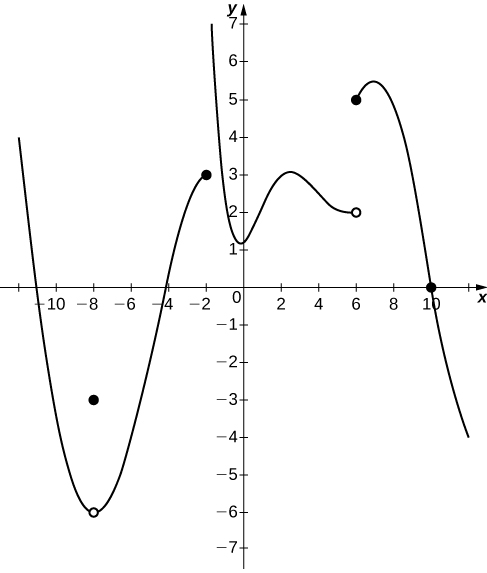
\includegraphics[scale=1]{images/Figure 2.2.1.jpg}
\end{center}
\end{example}

% =========================================================================

\newpage 
\subsection{Limit Laws}

\newpage 
\subsection{Continuity}

\newpage 
\subsection{Definition of a Limit}